\documentclass{article}
\usepackage[spanish]{babel}
\usepackage{amsmath}
\usepackage{amsthm}
\usepackage{amssymb}
\usepackage{ dsfont }
\usepackage{adjustbox}
\usepackage[shortlabels]{enumitem}
\usepackage[margin=1in]{geometry}
\usepackage{caption}
\usepackage[nocheck]{fancyhdr}
\usepackage[most]{tcolorbox}
\usepackage{xcolor}
\usepackage{biblatex}
\usepackage{listings}
\usepackage{algorithm}
\usepackage{algpseudocode}
\usepackage{pgffor}
\usepackage{import}
\usepackage{MnSymbol,wasysym}
\usepackage{graphicx}
\usepackage{float}
\usepackage[utf8]{inputenc}
\usepackage{longtable}
\usepackage{array}
\usepackage[spanish]{babel}
\usepackage{geometry}
\usepackage{tabularx}
\usepackage{tcolorbox}
\usepackage{pdfpages}



\renewcommand{\qedsymbol}{$\blacksquare$}

\addto\captionsspanish{\renewcommand{\proofname}{\normalfont{\textbf{Solución}}}}

\addbibresource{references.bib}

\thispagestyle{fancy}
\rhead{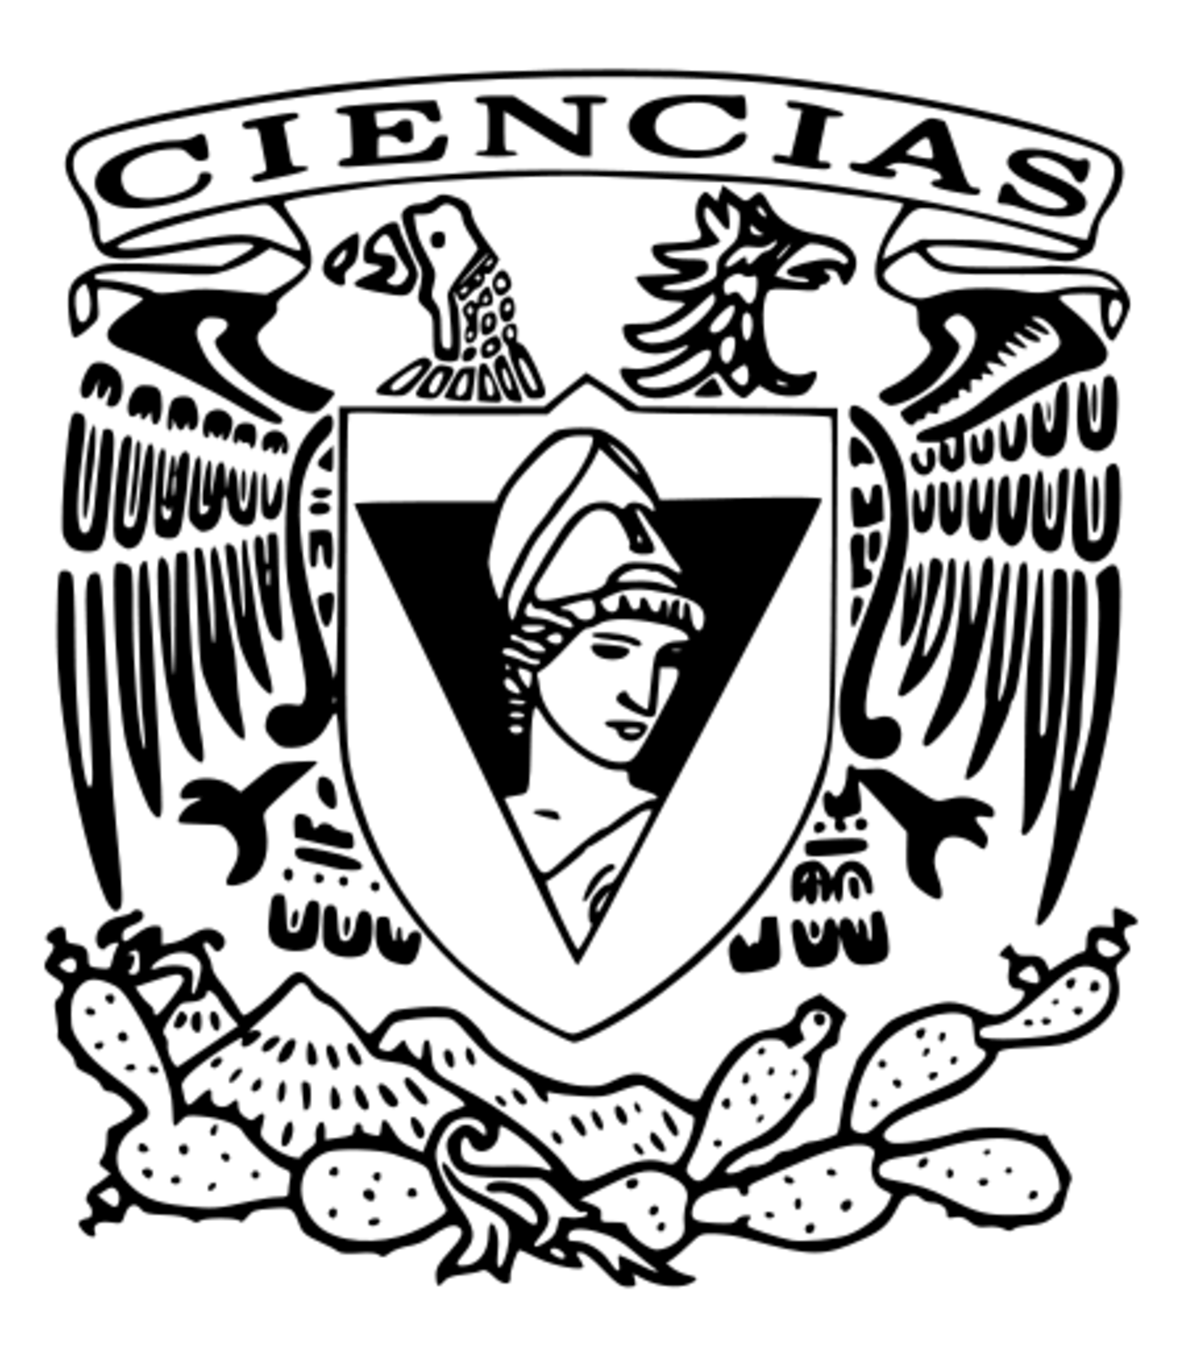
\includegraphics[scale=0.07]{Logo_FC.png}}
\lhead{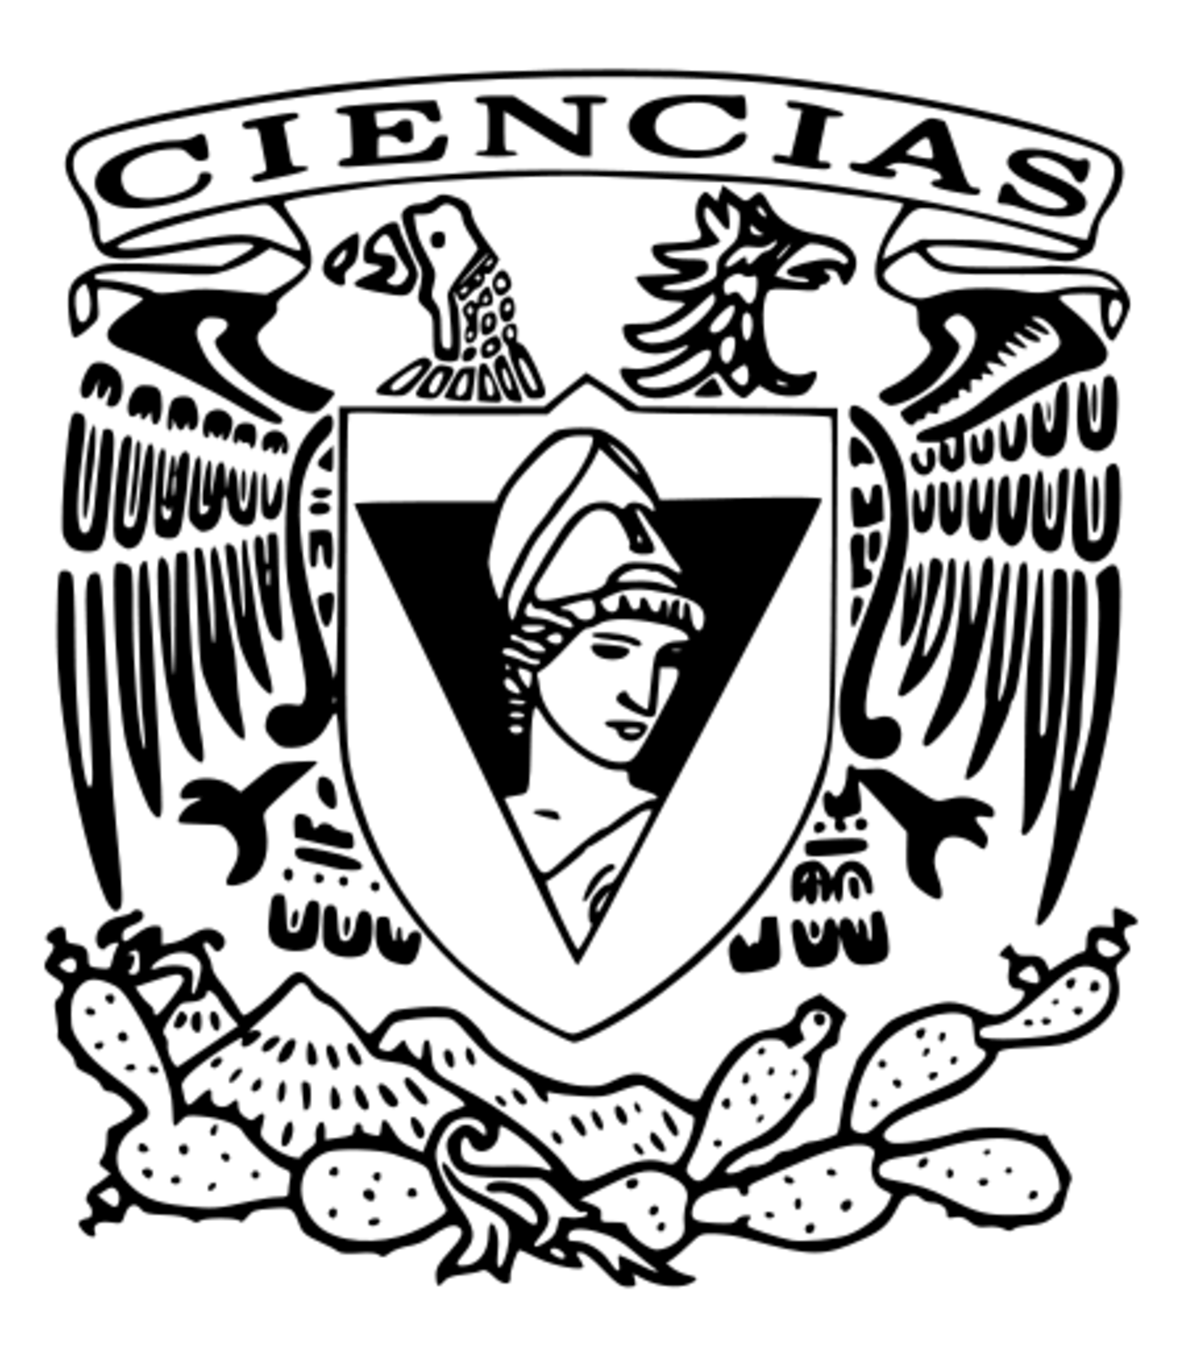
\includegraphics[scale=0.065]{Logo_FC.png}}
\chead{\large\textbf{Gestión de Inventario y Punto de Venta} \\
\textbf{Facultad de Ciencias - UNAM}\\
\textsc{Ingeniería de Software}\\
\textsc{Febrero 2025}\\
\centering{Un sistema de software para administrar de manera\\ eficiente un comercio.}
}
\renewcommand{\headrulewidth}{1pt}
%\pagenumbering{gobble}
\AtBeginDocument{\vspace*{4.2\baselineskip}}

\definecolor{FireBlue}{rgb}{0,0, 54.5}
\definecolor{Salmon}{rgb}{	80.8, 93.7, 100}

\begin{document}

\tableofcontents



\newpage
\section{Modulos Principales}

\subsection{Producto}
El producto administrará los artículos disponibles en la tienda, permitiendo su creación, edición y categorización, así como la asignación de precios y descripciones. Mantendrá la información detallada de cada ítem en el inventario.

\subsection{Tienda}
La tienda facilitará la configuración y administración general del establecimiento, incluyendo información comercial, ajustes operativos y personalización de la plataforma. Será la entidad que centraliza la operación completa del negocio.

\subsection{Punto de venta}
El punto de venta será el encargado de administrar las operaciones directas con el cliente. Permitirá generar ventas, cancelaciones, devoluciones, así como gestionar aperturas y cierres de caja. Coordinará el procesamiento de transacciones comerciales e integrará la información con otros módulos del sistema.

\subsection{Gestion de inventario}
La gestión de inventario controlará el stock de productos, permitiendo realizar ajustes en las existencias, registrar movimientos y gestionar el abastecimiento de la tienda. Mantendrá actualizada la información sobre disponibilidad de productos y coordinará con otros módulos para reflejar los cambios en tiempo real.

\subsection{Venta}
La venta se encargará del procesamiento de transacciones comerciales dentro del sistema, incluyendo la generación de tickets, cálculo de totales y aplicación de descuentos o promociones. Registrará cada operación comercial realizada en el punto de venta.

\subsection{Cliente}
El cliente permitirá administrar la base de datos de usuarios finales, facilitando el registro de información personal, historial de compras y preferencias para mejorar la experiencia del usuario. Mantendrá actualizada la información de contacto y comportamiento de compra.

\subsection{Proveedor}
El proveedor manejará la información de los suministradores de productos, permitiendo registrar, actualizar y consultar datos de contacto, historial de compras y acuerdos comerciales. Facilitará la gestión de relaciones con las empresas que abastecen la tienda.

\subsection{Gesti\'on de usuarios}
La gestión de usuarios permitirá administrar las cuentas de los empleados y otros usuarios del sistema, definiendo roles y permisos según su nivel de acceso dentro de la tienda. Controlará quién puede realizar determinadas operaciones dentro del sistema.

\subsection{Notificaciones}
Las notificaciones serán responsables de enviar alertas y recordatorios a los destinatarios correspondientes según los eventos que lo activen. Dependiendo del tipo de evento, se generará una notificación específica, ya sea periódica, preventiva o de alerta inmediata.

\subsection{An\'alisis}
El análisis se encargará del procesamiento y análisis inteligente de la información disponible en el sistema, permitiendo obtener conocimientos útiles a partir de los datos almacenados. Proveerá predicciones sobre eventos futuros con base en datos históricos y generará recomendaciones para la toma de decisiones comerciales.

\subsection{DAO}
El DAO (Data Access Object) será el encargado de administrar todos los accesos a la base de datos, permitiendo la interacción entre la aplicación y el almacenamiento de datos de manera estructurada y eficiente. Proporcionará una capa de abstracción para las operaciones de datos.

\subsection{Reportes}
Los reportes generarán informes personalizados según los datos requeridos por el usuario, extrayendo y procesando la información relevante de la base de datos. Proporcionarán visibilidad sobre el desempeño histórico y actual de diversas áreas del negocio.\\

\newpage




\section{Tarjetas de responsabilidades}
\newcommand{\tarjeta}[3]{
\begin{tcolorbox}[colback=gray!10, colframe=black, width=1\textwidth, halign=center, title=#1]
\begin{tabularx}{\linewidth}{X}
\textbf{Responsabilidad:} \\
#2 \\
\textbf{Colaboradores:} \\
#3
\end{tabularx}
\end{tcolorbox}
}

\vspace{0.1cm}

\noindent\begin{minipage}[t]{0.48\textwidth}
\tarjeta{Punto de venta}{
\begin{itemize}
\item \texttt{int generarVenta();}
\item \texttt{boolean cancelarTransaccion();}
\item \texttt{float procesarDevolucion();}
\item \texttt{String generarCorte();}
\item \texttt{boolean iniciarApertura();}
\item \texttt{boolean ejecutarCierre();}
\end{itemize}
}{
\begin{itemize}
\item Gestión de usuarios
\item Venta
\end{itemize}
}
\end{minipage}
\hfill
\begin{minipage}[t]{0.48\textwidth}
\tarjeta{Cliente}{
\begin{itemize}
\item \texttt{int registrarCliente();}
\item \texttt{boolean modificarDatosCliente();}
\item \texttt{String mostrarInformacionCliente();}
\end{itemize}
}{
\begin{itemize}
\item Punto de Venta
\item Venta
\item Reportes
\end{itemize}
}
\end{minipage}

\vspace{0.5cm}

\noindent\begin{minipage}[t]{0.48\textwidth}
\tarjeta{Tienda}{
\begin{itemize}
\item \texttt{int registrarTienda();}
\item \texttt{boolean modificarDatosTienda();}
\item \texttt{boolean inicializarBaseDatos();}
\end{itemize}
}{
\begin{itemize}
\item Gestión de Inventarios
\item Gestión de usuarios
\end{itemize}
}
\end{minipage}
\hfill
\begin{minipage}[t]{0.48\textwidth}
\tarjeta{Proveedor}{
\begin{itemize}
\item \texttt{int crearProveedor();}
\item \texttt{boolean modificarProveedor();}
\item \texttt{String consultarProveedor();}
\end{itemize}
}{
\begin{itemize}
\item Gestión de Inventario
\end{itemize}
}
\end{minipage}

\vspace{0.5cm}

\noindent\begin{minipage}[t]{0.48\textwidth}
\tarjeta{Gestión de Inventario}{
\begin{itemize}
\item \texttt{boolean agregarProductos();}
\item \texttt{String categorizarProductos();}
\item \texttt{int actualizarExistencias();}
\end{itemize}
}{
\begin{itemize}
\item Producto
\item Tienda
\item Venta
\item Punto de venta
\end{itemize}
}
\end{minipage}
\hfill
\begin{minipage}[t]{0.48\textwidth}
\tarjeta{Gestión de Usuarios}{
\begin{itemize}
\item \texttt{int crearUsuario();}
\item \texttt{boolean modificarUsuario();}
\item \texttt{String consultarUsuario();}
\end{itemize}
}{
\begin{itemize}
\item Punto de venta
\item Gestión de Inventario
\item Tienda
\end{itemize}
}
\end{minipage}

\vspace{0.5cm}

\noindent\begin{minipage}[t]{0.48\textwidth}
\tarjeta{Reportes}{
\begin{itemize}
\item \texttt{String[] generarHistoricos();}
\item \texttt{String mostrarHistorialUsuarios();}
\end{itemize}
}{
\begin{itemize}
\item Venta
\item Gestión de Inventario
\item Producto
\item Proveedor
\item Usuarios
\item Clientes
\end{itemize}
}
\end{minipage}
\hfill
\begin{minipage}[t]{0.48\textwidth}
\tarjeta{Análisis}{
\begin{itemize}
\item \texttt{String obtenerAnalisisPredictivo();}
\item \texttt{String[] mostrarTendencias();}
\item \texttt{String[] generarRecomendaciones();}
\item \texttt{float estimarGanancias();}
\end{itemize}
}{
\begin{itemize}
\item Reportes
\item Notificaciones
\end{itemize}
}
\end{minipage}

\vspace{0.5cm}

\noindent\begin{minipage}[t]{0.48\textwidth}
\tarjeta{Producto}{
\begin{itemize}
\item \texttt{int añadirProducto();}
\item \texttt{boolean modificarProducto();}
\item \texttt{boolean eliminarProducto();}
\item \texttt{String mostrarDetallesProducto();}
\end{itemize}
}{
\begin{itemize}
\item Venta
\item Gestión de Inventario
\item Proveedor
\end{itemize}
}
\end{minipage}
\hfill
\begin{minipage}[t]{0.48\textwidth}
\tarjeta{Venta}{
\begin{itemize}
\item \texttt{int registrarVenta();}
\item \texttt{boolean modificarVenta();}
\item \texttt{String consultarVenta();}
\end{itemize}
}{
\begin{itemize}
\item Punto de venta
\item Producto
\item Venta
\item Cliente
\end{itemize}
}
\end{minipage}

\vspace{0.5cm}

\noindent\begin{minipage}[t]{0.48\textwidth}
\tarjeta{Notificaciones}{
\begin{itemize}
\item \texttt{boolean enviarNotificacion();}
\end{itemize}
}{
\begin{itemize}
\item Producto
\item Gestión de Inventario
\item Venta
\end{itemize}
}
\end{minipage}
\hfill
\begin{minipage}[t]{0.48\textwidth}
\tarjeta{DAO}{
\begin{itemize}
\item \texttt{String[] ejecutarConsulta();}
\item \texttt{boolean realizarActualizacion();}
\end{itemize}
}{
\begin{itemize}
\item Gestión de usuarios
\item Gestión de Inventario
\item Reportes
\item Producto
\item Venta
\item Cliente
\item Tienda
\end{itemize}
}
\end{minipage}

\clearpage
\section{Diagrama Entidad-Relaci\'on}

\subsection{Sistema de usuarios administradores de tiendas}
\begin{figure}[h]
\centering
\includegraphics[width=0.6\textwidth]{assets/part1.png}
\end{figure}

\subsection{Registro de movimientos de inventario}
\begin{figure}[h]
\centering
\includegraphics[width=0.45\textwidth]{assets/part2.png}
\end{figure}

\newpage

\subsection{Punto de Venta o Caja Registradora}
\begin{figure}[h]
\centering
\includegraphics[width=1.1\textwidth]{assets/part3.png}
\end{figure}

\newpage
\subsection{Sistema de permisos modulares}
\begin{figure}[h]
\centering
\includegraphics[width=0.6\textwidth]{assets/part4.png}
\end{figure}

\newpage
\subsection{Registro de compras}
\begin{figure}[h]
\centering
\includegraphics[width=1\textwidth]{assets/part5.png}
\end{figure}


\subsection{Asociación de clientes con las ventas}
\begin{figure}[h]
\centering
\includegraphics[width=0.9\textwidth]{assets/part6.png}
\end{figure}

\newpage
\subsection{Categorización de productos}
\begin{figure}[h]
\centering
\includegraphics[width=0.7\textwidth]{assets/part7.png}
\end{figure}
\clearpage
\includepdf[landscape=true]{assets/ER.pdf}

\newpage
\section{Planos de p\'aginas}

\subsection{Ingreso}
\begin{figure}[h]
\centering
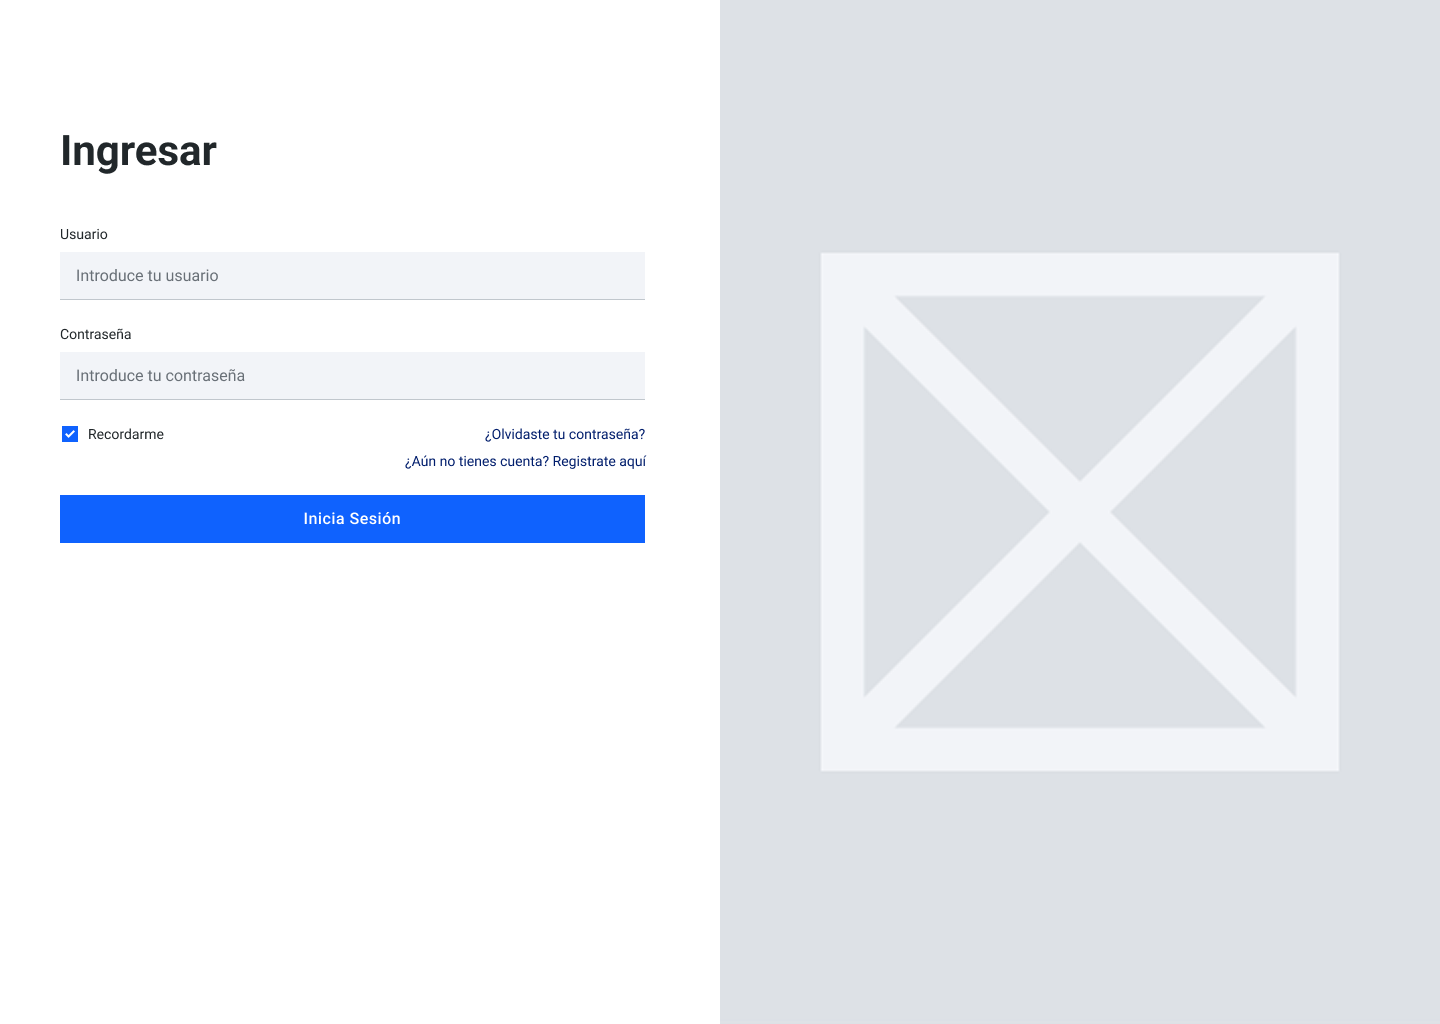
\includegraphics[width=0.7\textwidth]{wireframe/Ingreso.png}
\end{figure}

\subsection{Registro}
\begin{figure}[h]
\centering
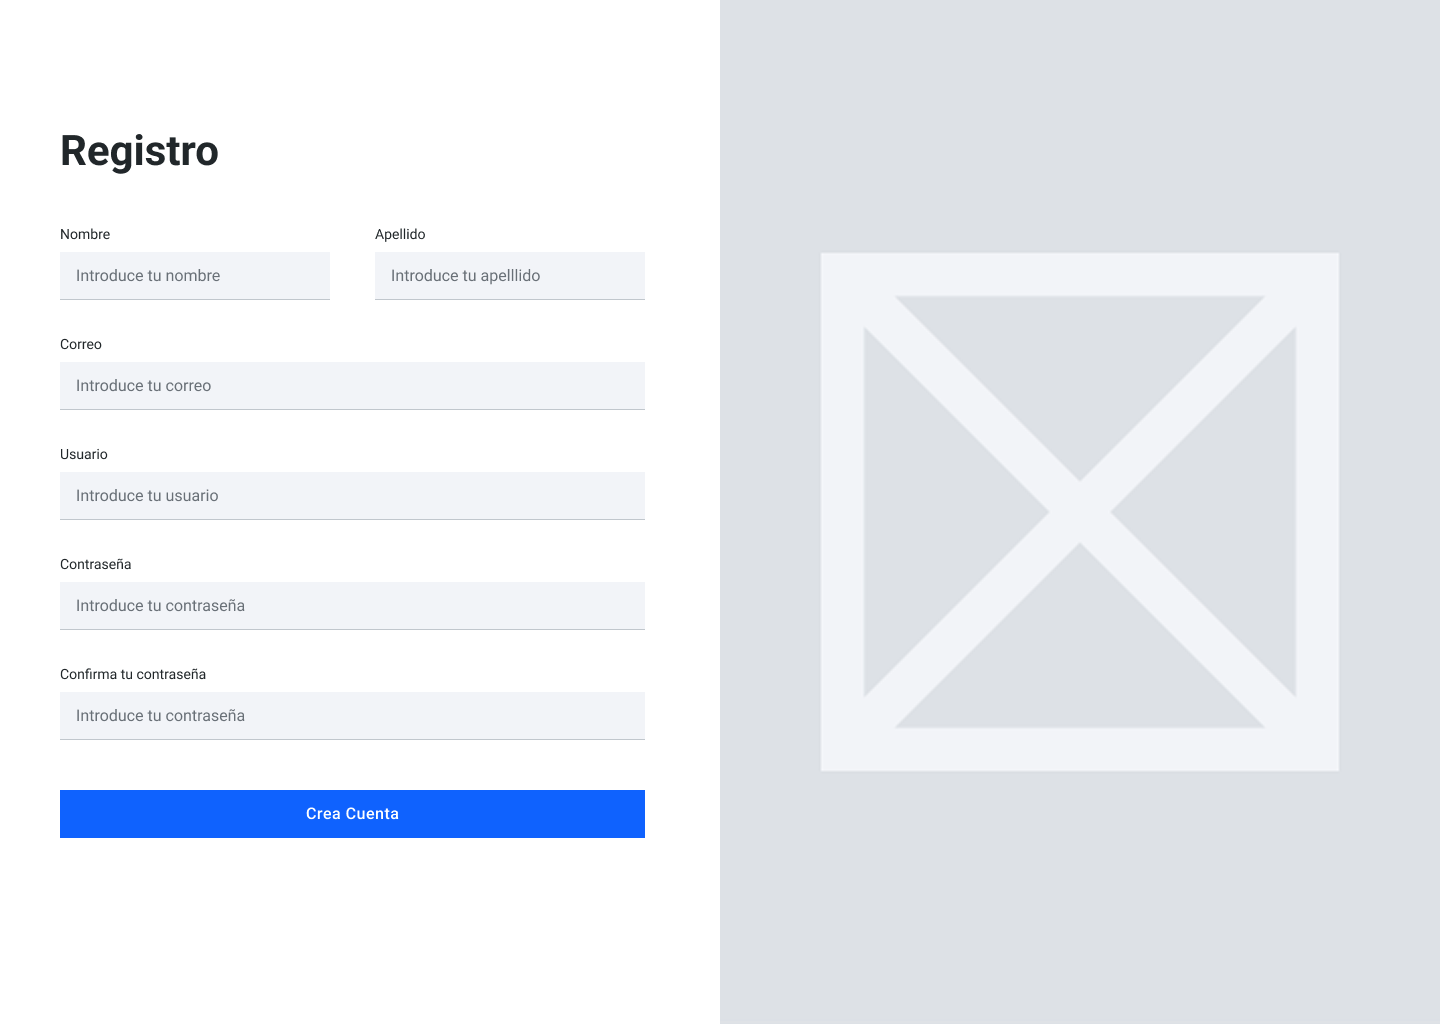
\includegraphics[width=0.7\textwidth]{wireframe/Registro.png}
\end{figure}

\newpage
\subsection{Centro de administraci\'on (Vista para superusuario)}
\begin{figure}[h]
\centering
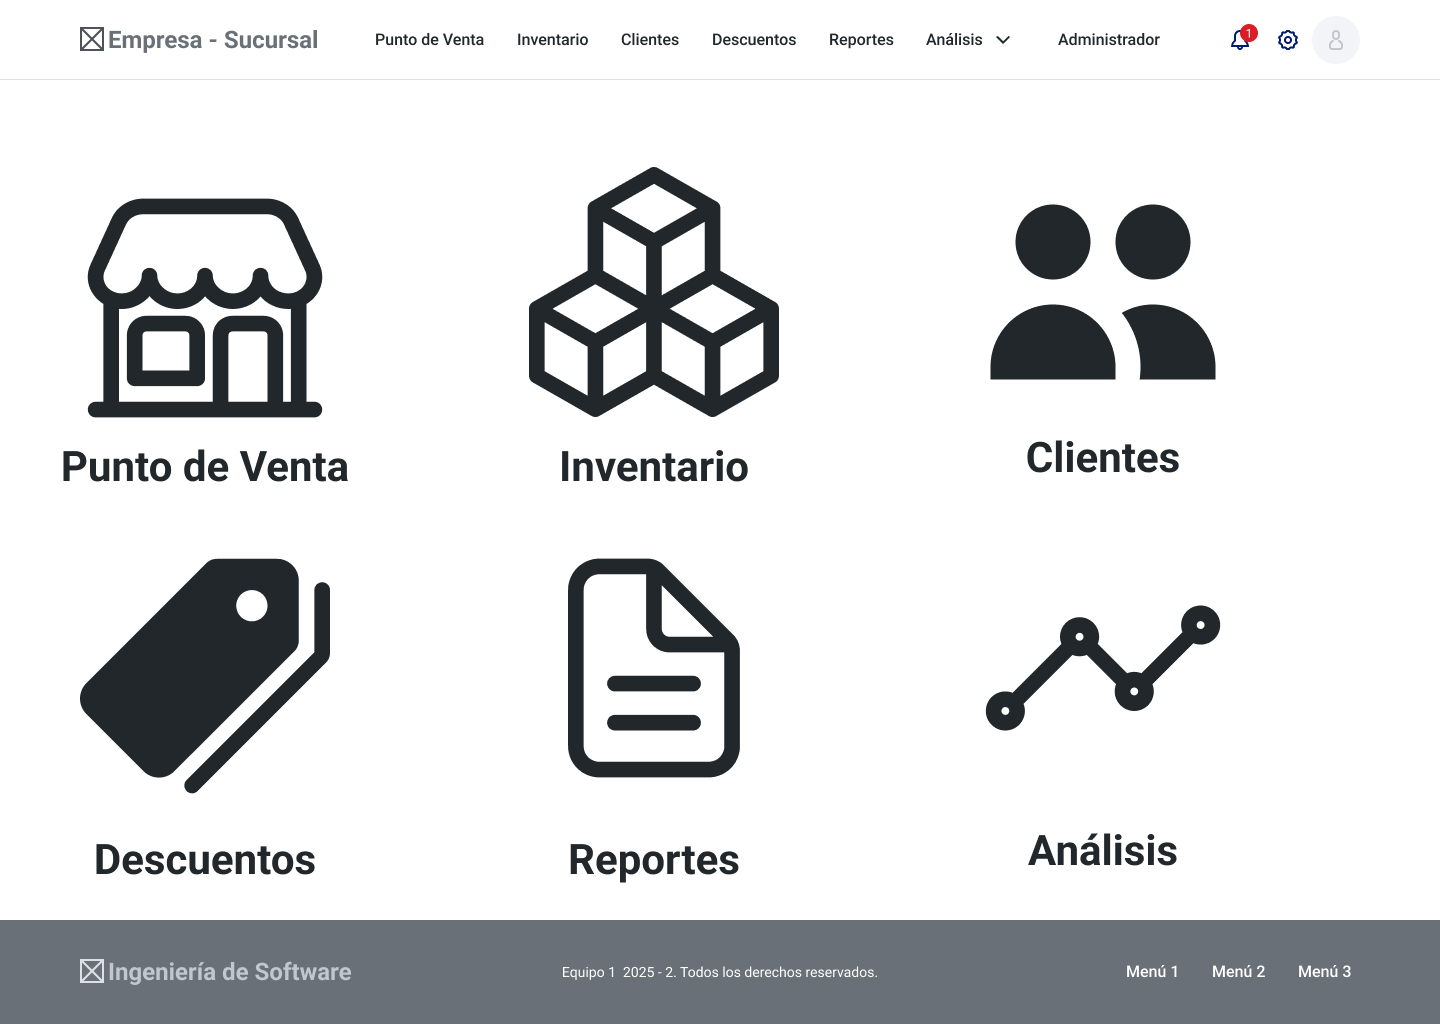
\includegraphics[width=0.7\textwidth]{wireframe/Centro Administrador.png}
\end{figure}


\subsection{Centro de administracion (Vista para usuario con restricci\'ones)}
\begin{figure}[h]
\centering
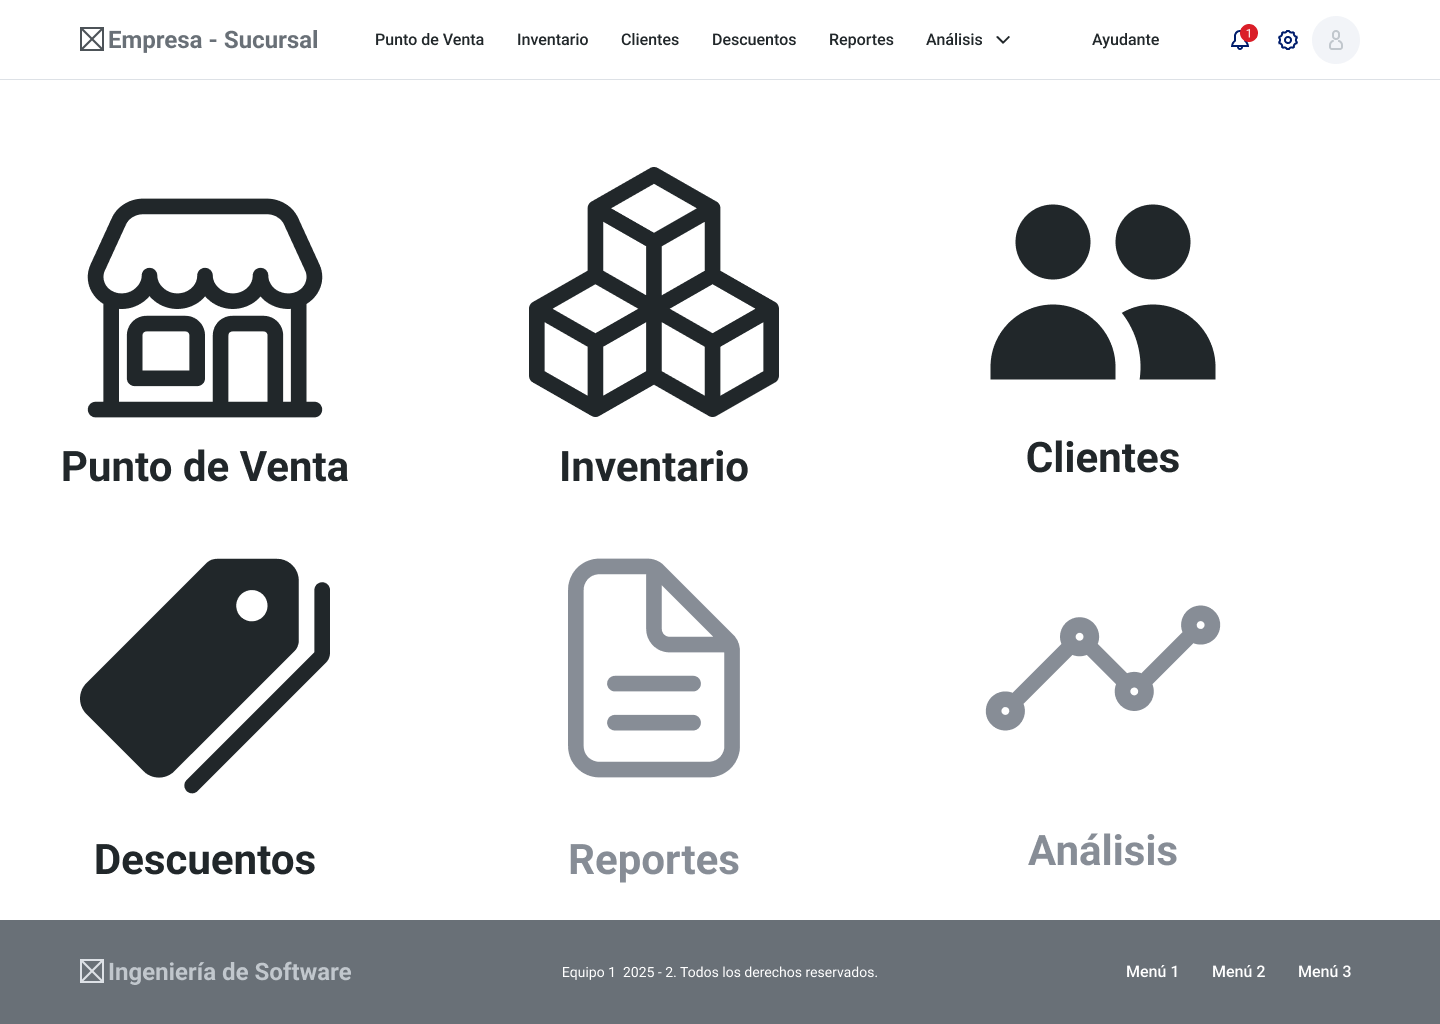
\includegraphics[width=0.7\textwidth]{wireframe/Centro Ayudante.png}
\end{figure}

\newpage
\subsection{Punto de venta}
\begin{figure}[h]
\centering
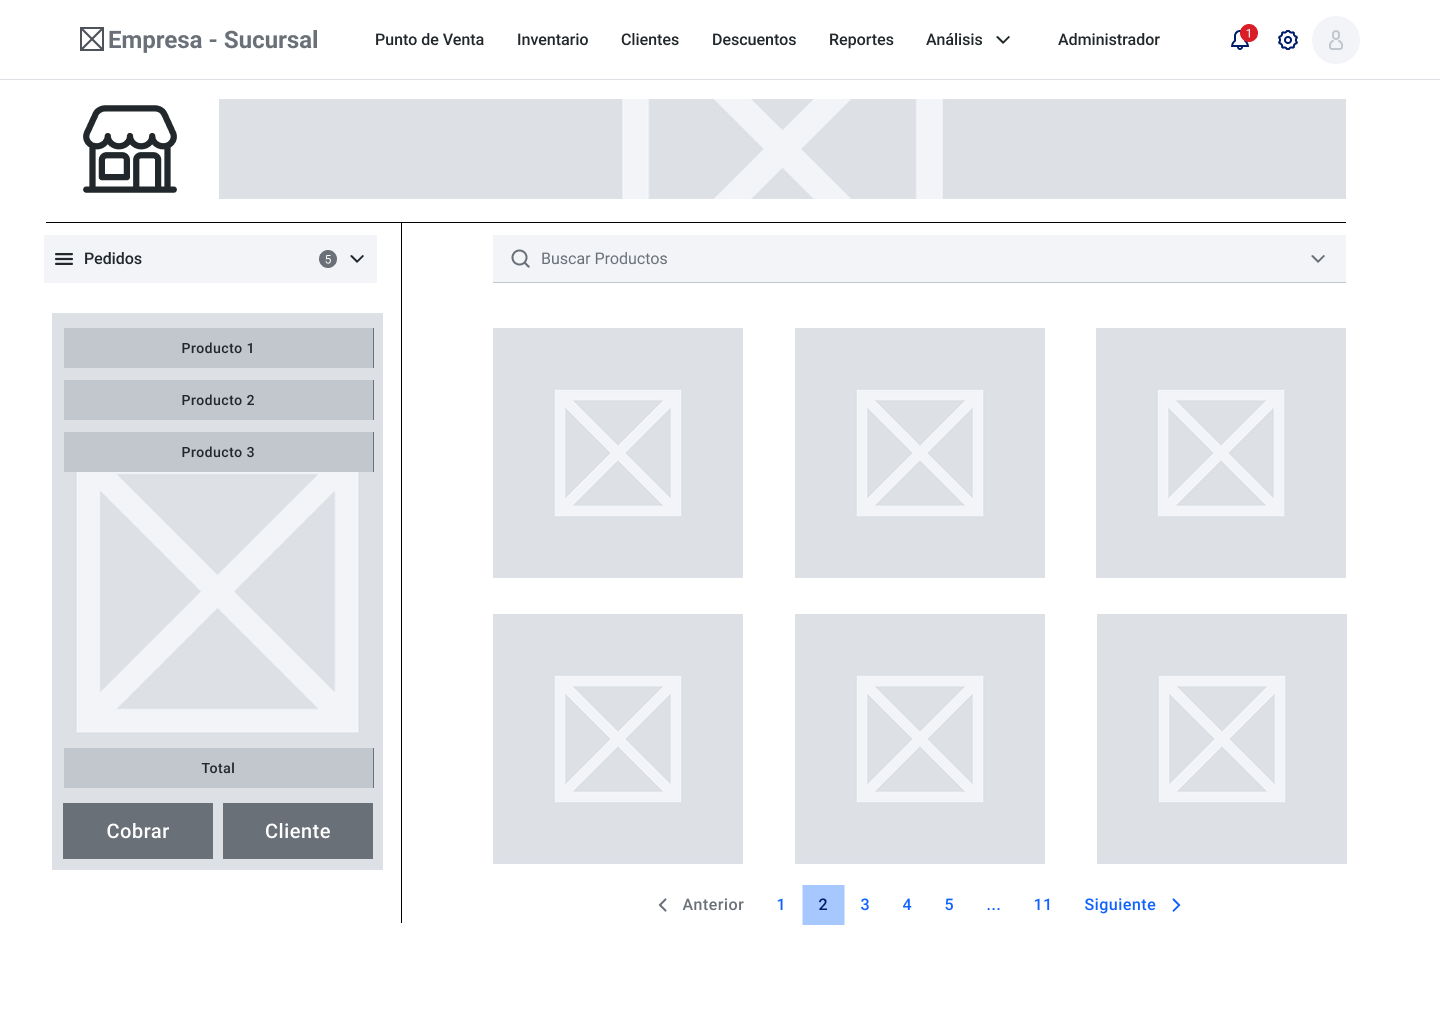
\includegraphics[width=0.7\textwidth]{wireframe/Punto de Venta.png}
\end{figure}

\subsection{Inventario}
\begin{figure}[h]
\centering
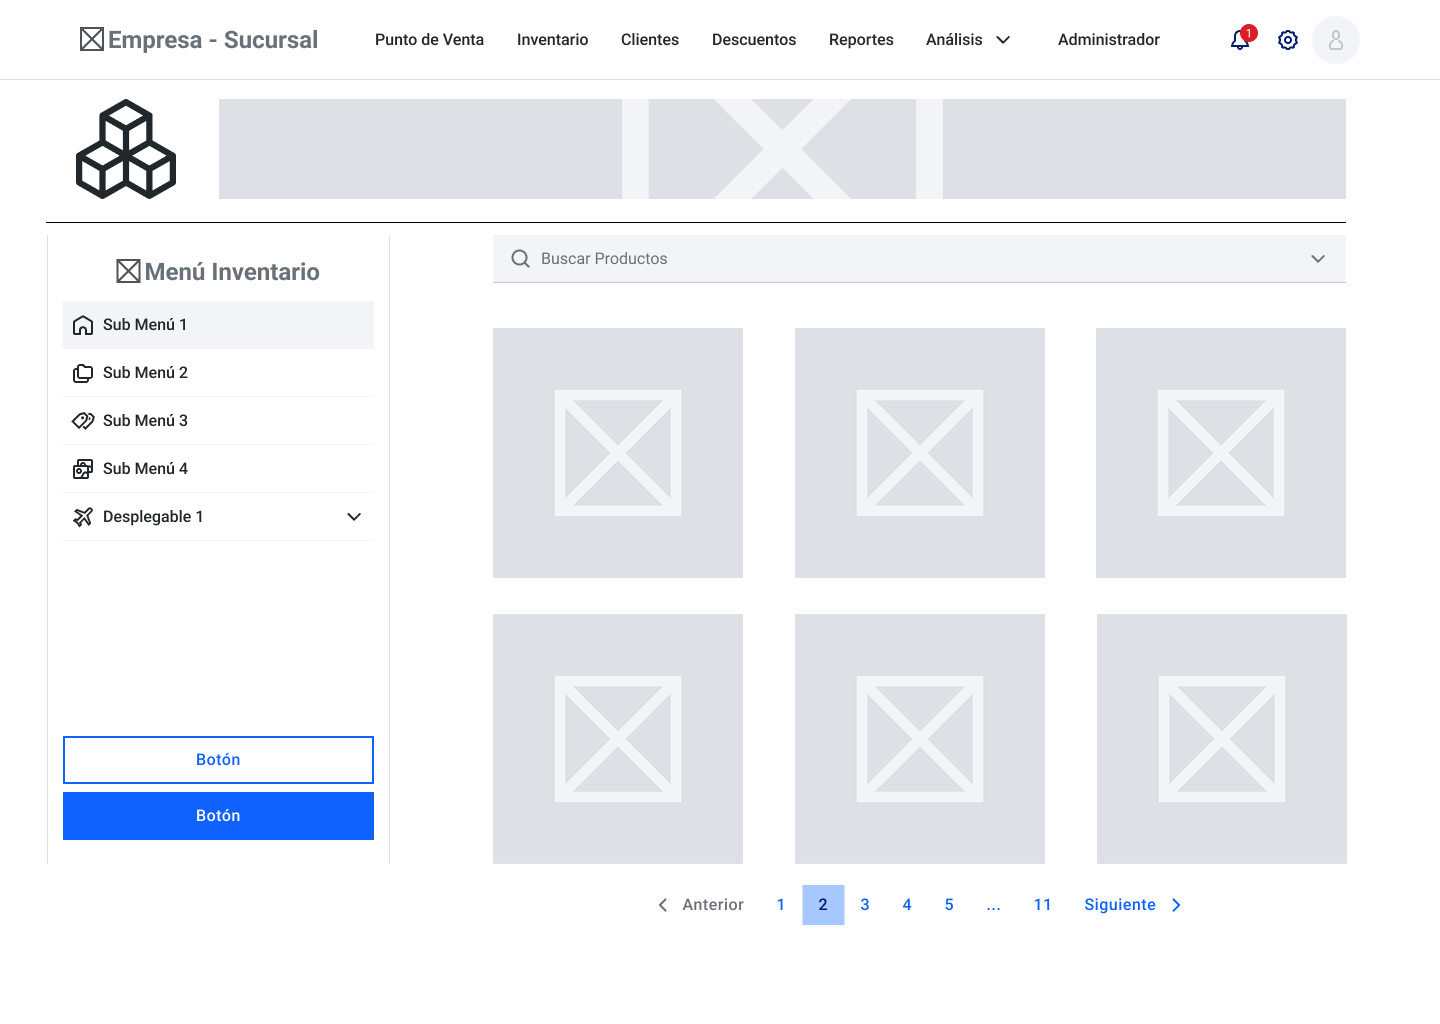
\includegraphics[width=0.7\textwidth]{wireframe/Inventario.png}
\end{figure}

\newpage
\subsection{Clientes}
\begin{figure}[h]
\centering
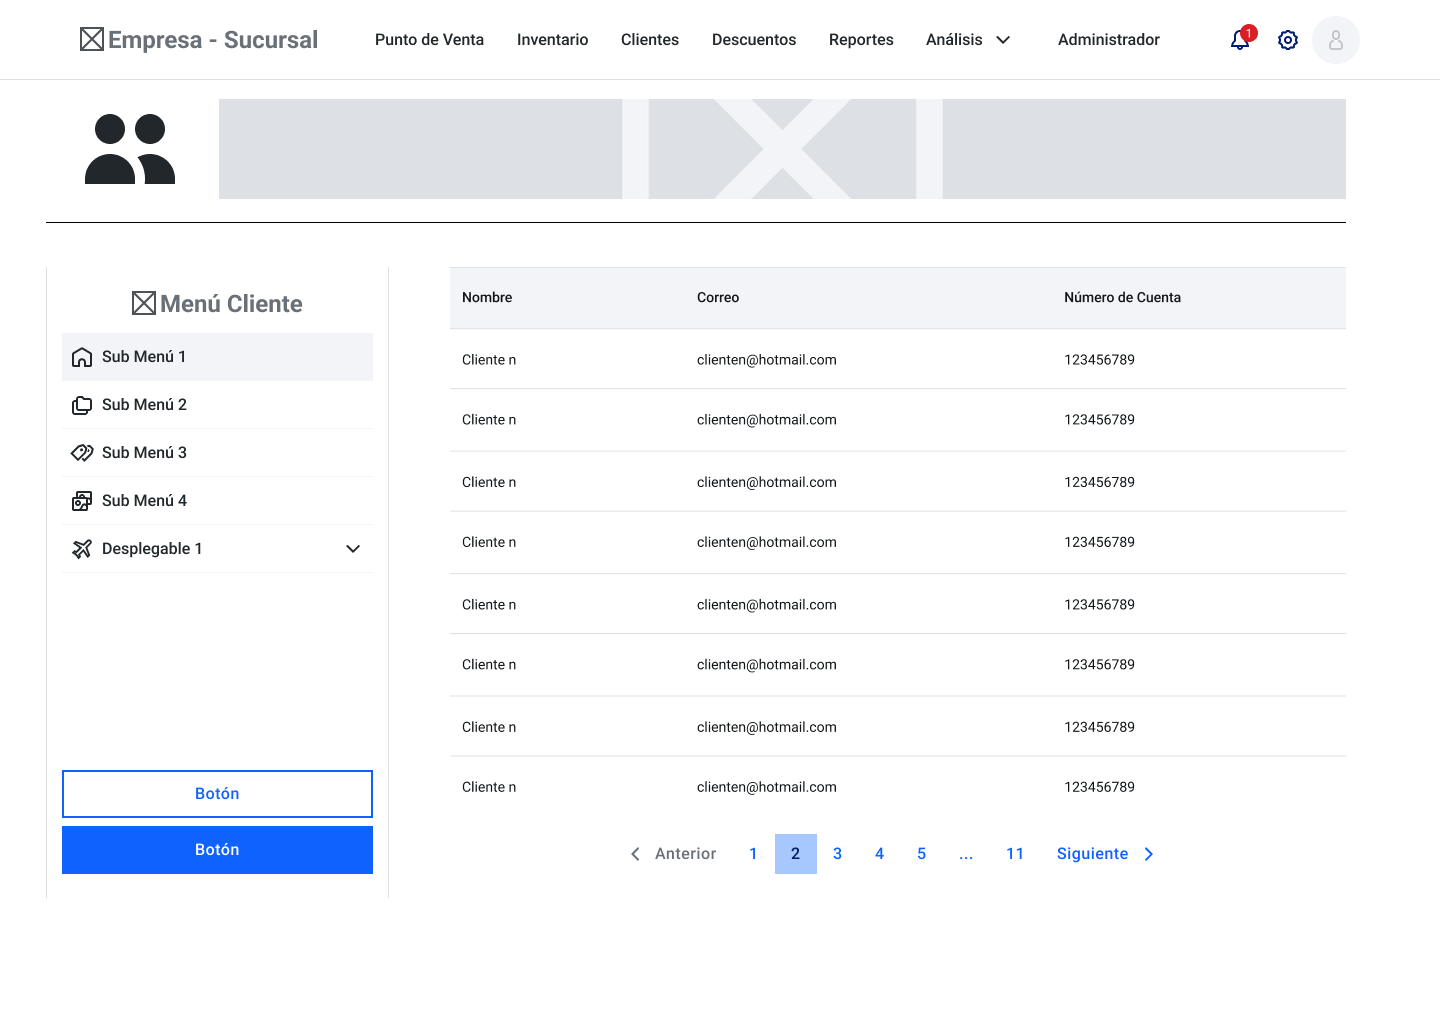
\includegraphics[width=0.7\textwidth]{wireframe/Clientes.png}
\end{figure}


\subsection{Descuentos}
\begin{figure}[h]
\centering
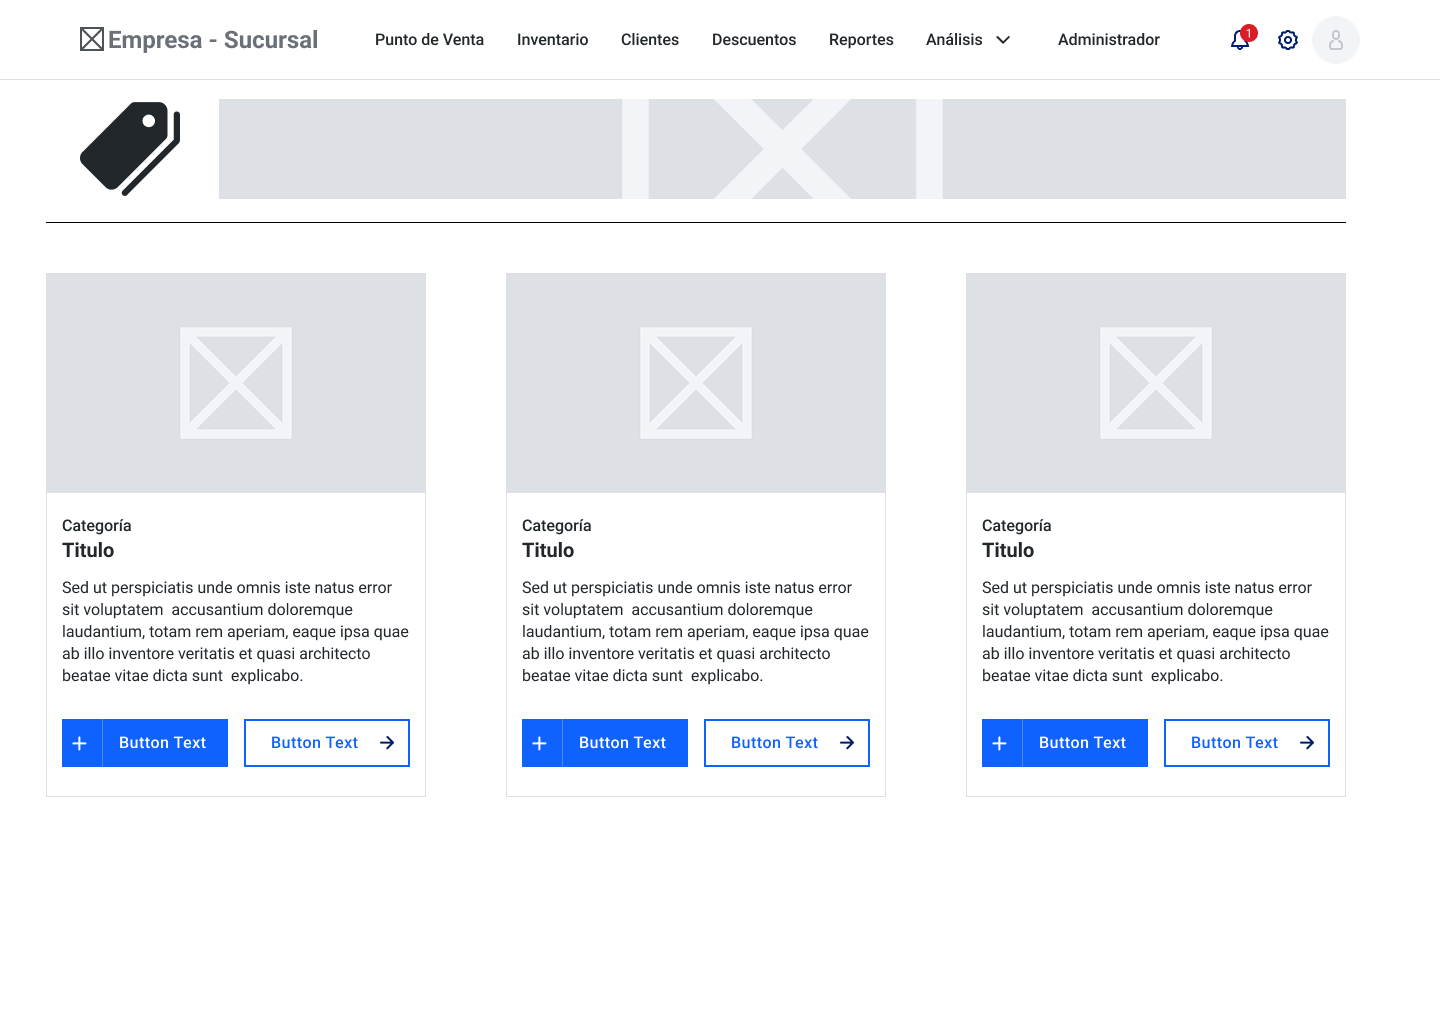
\includegraphics[width=0.7\textwidth]{wireframe/Descuentos.png}
\end{figure}

\newpage

\subsection{Reportes}
\begin{figure}[h]
\centering
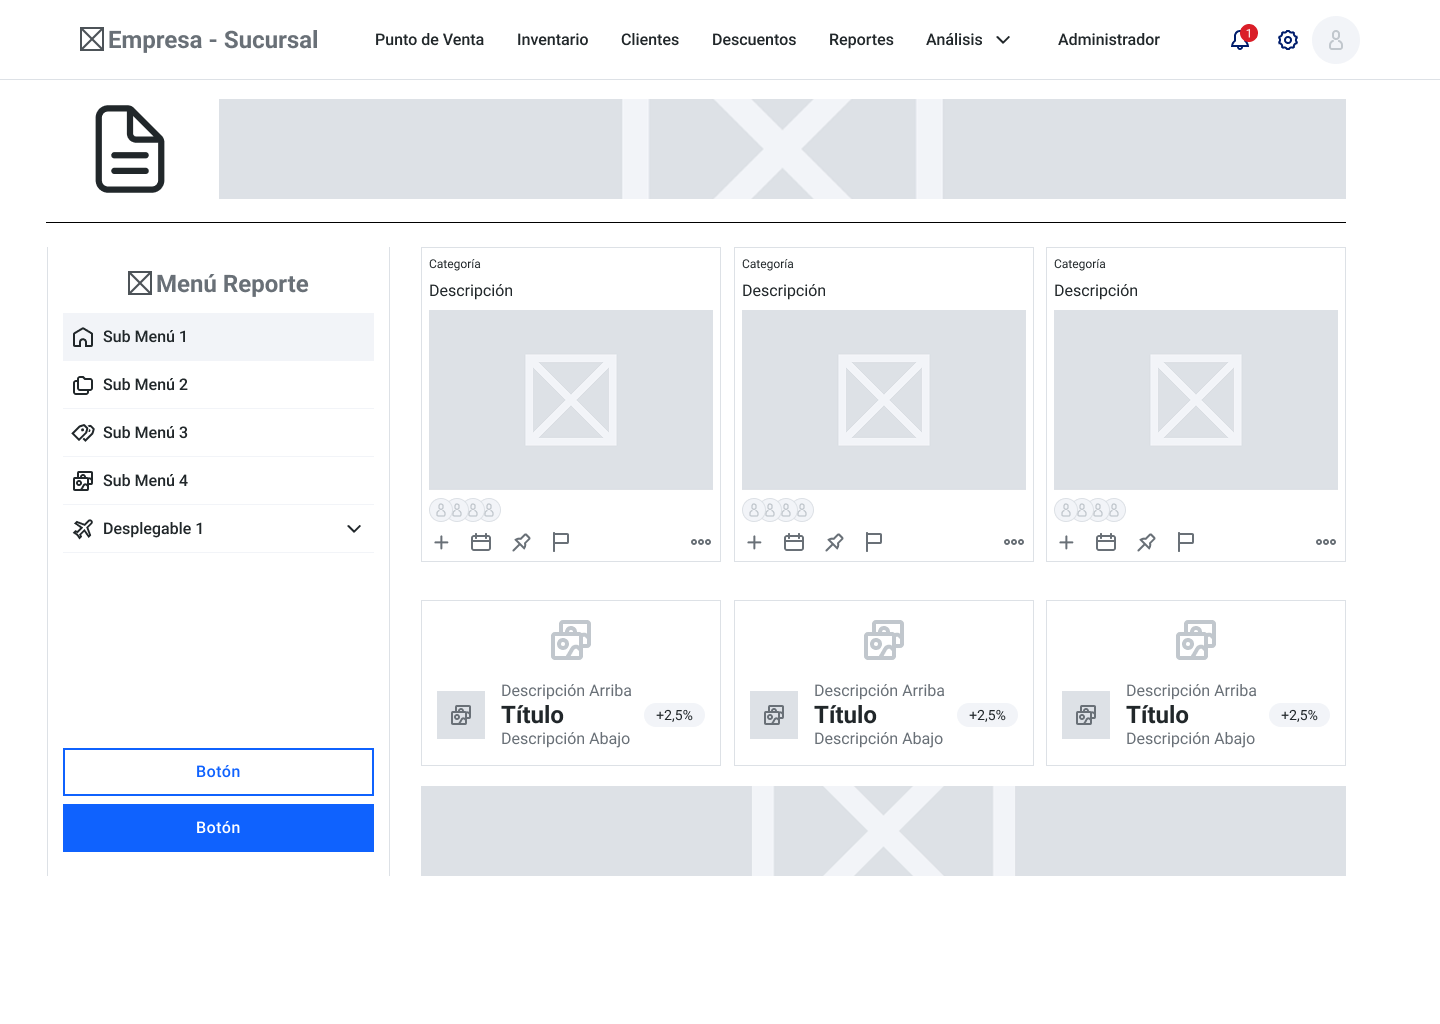
\includegraphics[width=0.7\textwidth]{wireframe/Reportes.png}
\end{figure}


\subsection{An\'alisis}
\begin{figure}[h]
\centering
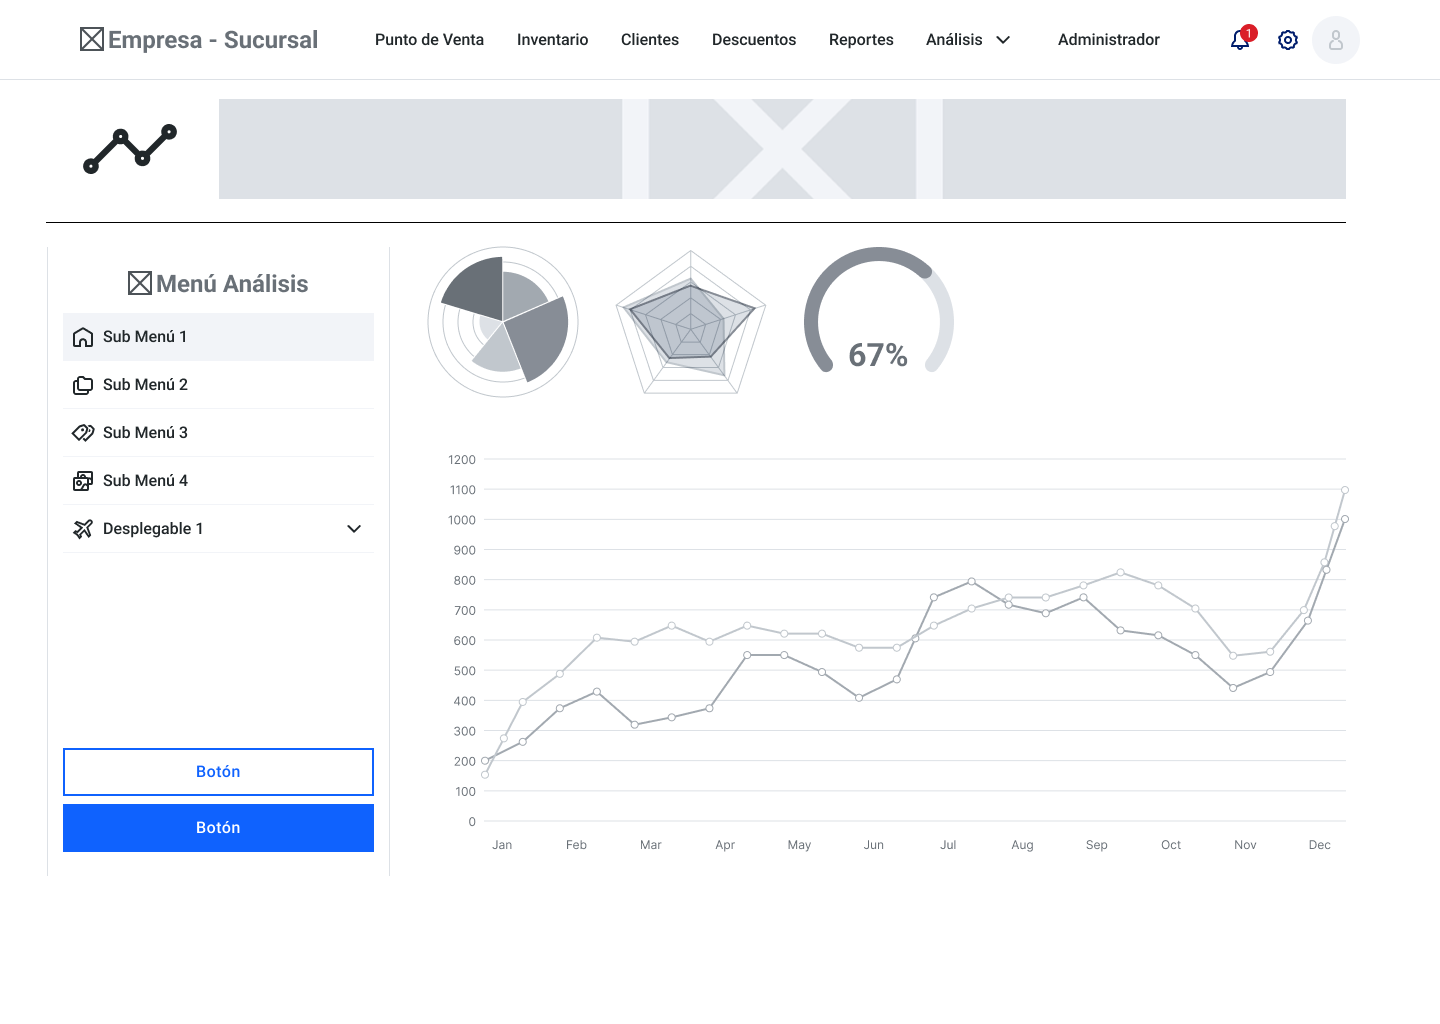
\includegraphics[width=0.7\textwidth]{wireframe/Analisis.png}
\end{figure}




\end{document}